\documentclass[11pt]{article}
\usepackage[margin=1in]{geometry}
\usepackage{amsmath,amssymb,bbm}
\usepackage{float,color}
\usepackage{hyperref}
\usepackage{booktabs}
\usepackage{placeins}
\usepackage{graphicx}
\usepackage[
backend=biber,
style=bwl-FU,
sorting=ynt
]{biblatex}
\addbibresource{../main.bib}

%%%%% Math Commands %%%%%
\DeclareMathOperator*{\argmax}{arg\,max}
\DeclareMathOperator*{\argmin}{arg\,min}

\newtheorem{fact}{Fact}
\newtheorem{lemma}{Lemma}
\newtheorem{theorem}[lemma]{Theorem}
\newtheorem{defn}[lemma]{Definition}
\newtheorem{assumption}[lemma]{Assumption}
\newtheorem{corollary}[lemma]{Corollary}
\newtheorem{prop}[lemma]{Proposition}
\newtheorem{exercise}[lemma]{Exercise}
\newtheorem{claim}[lemma]{Claim}
\newtheorem{remark}[lemma]{Remark}
\newtheorem{prob}{Problem}
\newtheorem{conjecture}{Conjecture}

\newenvironment{note}[1]{\medskip\noindent \textbf{#1:}}%
        {\medskip}

\newenvironment{proof}{\vspace{-0.05in}\noindent{\bf Proof:}}%
        {\hspace*{\fill}$\Box$\par}
\newenvironment{proofsketch}{\noindent{\bf Proof Sketch.}}%
        {\hspace*{\fill}$\Box$\par\vspace{4mm}}
\newenvironment{proofof}[1]{\smallskip\noindent{\bf Proof of #1.}}%
        {\hspace*{\fill}$\Box$\par}

\newcommand{\etal}{{\em et al.}\ }
\newcommand{\assign}{\leftarrow}
\newcommand{\eps}{\epsilon}

\newcommand{\opt}{\textrm{\sc OPT}}
\newcommand{\script}[1]{\mathcal{#1}}
\newcommand{\ceil}[1]{\lceil #1 \rceil}
\newcommand{\floor}[1]{\lfloor #1 \rfloor}

%%%%% Subsubsubsection definition %%%%%
\usepackage{titlesec}
\titleclass{\subsubsubsection}{straight}[\subsection]

\newcounter{subsubsubsection}[subsubsection]
\renewcommand\thesubsubsubsection{\thesubsubsection.\arabic{subsubsubsection}}
\renewcommand\theparagraph{\thesubsubsubsection.\arabic{paragraph}} % optional; useful if paragraphs are to be numbered

\titleformat{\subsubsubsection}
  {\normalfont\normalsize\bfseries}{\thesubsubsubsection}{1em}{}
\titlespacing*{\subsubsubsection}
{0pt}{3.25ex plus 1ex minus .2ex}{1.5ex plus .2ex}

\makeatletter
\renewcommand\paragraph{\@startsection{paragraph}{5}{\z@}%
  {3.25ex \@plus1ex \@minus.2ex}%
  {-1em}%
  {\normalfont\normalsize\bfseries}}
\renewcommand\subparagraph{\@startsection{subparagraph}{6}{\parindent}%
  {3.25ex \@plus1ex \@minus .2ex}%
  {-1em}%
  {\normalfont\normalsize\bfseries}}
\def\toclevel@subsubsubsection{4}
\def\toclevel@paragraph{5}
\def\toclevel@paragraph{6}
\def\l@subsubsubsection{\@dottedtocline{4}{7em}{4em}}
\def\l@paragraph{\@dottedtocline{5}{10em}{5em}}
\def\l@subparagraph{\@dottedtocline{6}{14em}{6em}}
\makeatother

\setcounter{secnumdepth}{4}
\setcounter{tocdepth}{4}

\title{Agricultural Index Insurance Design: An Optimization Approach}
\author{José I. Velarde Morales}

\begin{document}
\maketitle
\tableofcontents

\section{Introduction}
Lack of access to credit and insurance is often cited as a significant factor hindering agricultural productivity in developing countries. Nearly two thirds of the world's poor are employed in agriculture, and addressing this problem could have significant welfare implications. Agricultural insurance is, even in the best circumstances, a hard problem. Many of the features one would want (independent units, uncorrelated risk, etc) are missing in this context. When considering insurance in developing countries, the problem becomes even harder because of verification costs. Traditionally, whenever an adverse event happens, the insured party contacts the insurer, and the insurer verifies the claim and issues a payout. However, agriculture in developing countries is often characterized by many small farmers spread out over hard to reach regions. This makes verification prohibitively costly. Additionally, the presence of correlated risks makes insurance more expensive because it makes large payouts more likely. Intuitively, if one farmer is affected by a drought, it is likely that other farmers were also affected. If large payouts are more likely, the insurer must have larger reserves in order to maintain solvency. 

Researchers developed index insurance as a less costly way to offer insurance in developing countries. In index insurance, an index (or statistic) is created using easily observable quantities, and it is used to determine whether the insured party suffered an adverse event. In the past, indices have been constructed using rainfall, weather, and satellite images. If the index falls below a pre-determined threshold, the insurance company automatically issues out payments to the insured. This allows the insurance company to circumvent the issue of verification, moral hazard, and adverse selection, since the actions of individual farmers cannot affect the index. Even though index insurance has proved to be a less costly way of providing insurance for small farmers, it has been difficult to scale up. There are several problems with index insurance. One of the main problems is low take up: farmers are often unwilling to purchase the insurance at market prices. Another problem, as previously mentioned, is the cost. The purpose of this project is to make this insurance less costly by improving the design of insurance contracts. The rest of this paper is organized as follows: Section 2 reviews the existing literature on index insurance, Section 3 describes our proposed approach, Section 4 describes our evaluation methods and results. We conclude with a brief discussion. 

\section{Literature Review}
\paragraph{Impact of Index Insurance} There are many studies that evaluate how access to index insurance impacts the behavior of farmers. Through a randomized evaluation in Northern Ghana, \cite{karlan2014agricultural} found that farmers shifted their production to riskier but potentially more profitable crops when they had access to index insurance. Similarly, \cite{cole2013barriers} found that farmers in India that had access to insurance were more likely to produce cash crops. \cite{mobarak2013informal} conducted experiments in several states in India and found that insured farmers were more likely to grow high-yield varieties of rice. Overall, there is evidence that index insurance reduces reliance on detrimental risk-coping strategies, increases investment, and leads to riskier, but more profitable production decisions (\cite{jensen2017agricultural}). 

\paragraph{Demand for Index Insurance} One of the largest barriers to the scale up and adoption of index insurance is low demand (\cite{jensen2017agricultural}). \cite{cole2013barriers} found that demand for index insurance is highly sensitive to price and liquidity constraints. When offered discounts, over $60\%$ of farmers opted to purchase the insurance product. They also found that cash grants made farmers more likely to purchase insurance. \cite{cai2020subsidy} found that subsidies and financial education increased take up of index insurance. \cite{casaburi2018time} tested the effect of liquidity constraints on demand. They reduced liquidity constraints by collecting premiums at harvest time (when farmers have more cash), instead of the standard pay-up-front scheme. They found that this payment scheme increased take up to $72\%$ from a baseline of $5\%$. 

\paragraph{Design of Index Insurance} There has been relatively little research done on the design of index insurance. In \cite{chantarat2013designing}, the authors describe the design of an index insurance for pastoralists in Northern Kenya. This insurance is based on a satellite based index, and is what is used in Kenya's Index Based Livestock Insurance (IBLI) program. In \cite{flatnes2018improving} the authors propose augmenting a traditional index insurance contract with the option for an audit. In this augmented contract, the insured farmer has the option to request an audit if they believe a payout should have been issued but wasn't. In \cite{jensen2019does}, the authors compare the welfare implications of using different satellite based indices for insuring pastoralists against drought. The method developed by \cite{chantarat2013designing} is used in all of these studies. There are also numerous non-academic publications describing the implementation of index insurance programs in different parts of the world (\cite{osgood2007designing},\cite{world2011weather},\cite{greatrex2015scaling}). From these papers describing the implementation of these programs, it appears that there is no a standard methodology for developing index insurance products. As stated in \cite{world2011weather}, "The reader should be aware that there is no single methodology in this field ... [this paper] describes an approach that has been used in a number of index pilot activities undertaken by the World Bank and its partners." 

\paragraph{Optimization Literature} In this work, we will be drawing from the literature on chance constrained programs (\cite{lagoa2005probabilistically}; \cite{charnes1958cost}). We also draw on the work on coherent risk measures (\cite{artzner1999coherent}), and work on the optimization of conditional value at risk by (\cite{rockafellar2000optimization}). Additionally, we use the results on convex approximations of chance constrained programs by (\cite{nemirovski2007convex}). 

\paragraph{Sustainable Operations} Mention Can Zhang's work, Somya Singhvi's work, Joan de Zegher, Priyank Arora, Beril Toktay, etc. 

\section{Optimization Approach}
  \subsection{Objective and Constraints}
    We conducted interviews with practitioners that had implemented index insurance programs in numerous countries (Malawi, Kenya, Senegal, Thailand, among others) to determine an appropriate objective for the model. Practitioners expressed that the ideal objective would be to minimize the probability that farmers' wealth would drop below a certain threshold. This is motivated/supported by the body of research on poverty traps. Poverty traps are typically defined as ``any self-reinforcing mechanism which causes poverty to persist'' (\cite{azariadis2005poverty}). The idea is that if a household's wealth drops below a certain threshold, they can be stuck there for a long time. For example, when faced with a negative income shock, a farmer might be forced to sell some of their productive assets. Without these productive assets, it can be very difficult to accumulate enough savings to re-purchase the productive asset, and the farmer might be stuck at the lower income level for a long time. One of the main purposes of insurance is to prevent these kinds of situations.  
    
    The most important constraints in practice are budget constraints and payout frequency constraints (\cite{osgood2007designing},\cite{world2011weather}). Price constraints are important from both the demand and supply side. On the supply side, insurers have strong preferences with regards to the premium of the product they offer. From the demand side, demand for index insurance is highly price elastic (\cite{jensen2017agricultural}). Payout frequency constraints are similarly from both the demand and supply sides. From the supply side, insurers don't want payout frequency to be too high, because there are fixed costs associated with issuing payouts. From the demand side, farmers generally have low demand for an instrument that pays out very infrequently (\cite{osgood2007designing}). Index insurance contracts normally define piecewise linear payout functions (\cite{world2011weather},\cite{chantarat2013designing}). Piecewise linear functions are popular because they are easy to explain, and have been found to work well in practice. Simplicity is an important feature, because low understanding of the product lowers demand for insurance (\cite{cai2020subsidy}).


  \subsection{Index Insurance Definition and Parameters}
    Index insurance generally involves an easily observable signal, $\theta$, that is used to predict the loss, $\hat{\ell}(\theta)$, of some agricultural product. For example, $\theta$ could be rainfall, and $\hat{\ell}(\theta)$ could be livestock mortality. Index insurance contracts normally have the form: $I(\hat{l}(\theta)) = \min \left \{\max \left \{0,a\hat{\ell}(\theta) + b \right \}, P \right \}$, where $P$ is the maximum payout, and $a,b$ are the contract parameters. For ease of notation, we will use $I(\theta)$ instead of $I(\hat{\ell}(\theta))$. The expected cost, $C(I(\theta))$ of an insurance contract, $I(\theta)$ for an insurer in a single period is: $C(I(\theta)) = \mathbb{E}[I(\theta)] + c_{\kappa} K(I(\theta))$, where $c_{\kappa}$ is the cost of holding capital, and $K$ is the amount of capital required to insure the contract. $K$ is set by regulators, and is meant to ensure that insurers have enough capital to fulfill their contractual obligations with high probability. One commonly used formula for $K$ is $K(I(\theta)) = CVaR_{1-\epsilon_P}\left ( I(\hat{l}(\theta)) \right ) - \mathbb{E}[I(\theta)]$ (\cite{mapfumo2017risk}). $\epsilon_P$ is set by regulators, and commonly used values are $\epsilon_P = 0.01$ or $\epsilon_P = 0.05$.  

  \subsection{CVaR Model}
    \subsubsection{Motivation}
      We want a model that minimizes the probability that wealth drops below a certain threshold, subject to a budget constraint. However, probabilistic objectives are generally non-convex. The probability that wealth drops below a certain threshold is a measure of the risk farmers face; we want a convex measure that will capture this risk. We use the Conditional Value at Risk $CVaR$ of the loss net of insurance as our measure of risk. 
  
    % \paragraph{Conditional Value at Risk} 
    \begin{defn}
      For a random variable $z$, representing loss, the $(1-\epsilon)$ Value at Risk $(VaR)$ is given by 
      \begin{align*}
        VaR_{1-\epsilon}(z) := \inf \left \{ t : P(z \leq t) \geq 1-\epsilon \right \}
      \end{align*}
    \end{defn}
  
    \begin{defn}
      For a random variable $z$, representing loss, the $(1-\epsilon)$ Conditional Value at Risk $(CVaR)$ is given by 
      \begin{align*}
        CVaR_{1-\epsilon}(z) := \mathbb{E}\left [z | z \geq VaR_{1-\epsilon}(z) \right ]
      \end{align*}
    \end{defn}
  
    Intuitively, the Conditional Value at Risk is the expected value of a loss given that it is above a certain threshold. It can also be thought of as measuring the worst outcomes. By minimizing the $CVaR$ of the net loss, we are focusing on improving farmers' wealth in the worst case scenarios, which is a key purpose of insurance. $CVaR$ has been extensively studied in the academic literature, and is also popular in practice (\cite{rockafellar2000optimization},\cite{rockafellar2002conditional},\cite{artzner1999coherent}). It also has the advantage of being convex, and thus amenable to optimization. This leads us to the following model: 
  
    \begin{align}
        \min_{a,b,\pi, K}  & \quad CVaR_{1-\epsilon}\left ( \ell + \pi - I(\theta) \right)\\
        \text{s.t.   }I(\theta) &= \min \{ (a\hat{\ell}(\theta) + b)^+,1\} \\
        \pi &= \mathbb{E}\left [ I(\theta) \right ] + c_{\kappa} K \\
        K &=  CVaR_{1-\epsilon}\left ( I(\theta)  - \mathbb{E}[I(\theta)] \right ) \label{cons-budget} \\
        \pi &\leq \overline{\pi}
    \end{align}
  
    Our objective is the conditional value at risk of the farmers' loss net of insurance. The first constraint specifies the piecewise linear structure of the contract, and the second constraint is the budget constraint. Recall that the total cost of insurance consists of payouts plus the cost of capital. The last constraint is just the definition of the required capital. 
    
    \subsubsection{Changes to constraints}
        To make the program convex, we replace $I(\theta)$ with conservative approximations where necessary, making sure that by doing so we still get a feasible solution. We use the following approximations of $I(\theta)$ to make the problem convex: 
      \begin{align*}
        \overline{I(\theta)} &\triangleq \max \left \{ 0,a\hat{\ell}(\theta) + b\right \} \\
        \underline{I(\theta)} &\triangleq \min \{ a\hat{\ell}(\theta) + b,1 \}\\
        &\implies \\
        \underline{I(\theta)} &\leq I(\theta) \leq \overline{I(\theta)}
        \end{align*}
    
        Note that $\overline{I(\theta)} \geq I(\theta)$ and $\overline{I(\theta)}$ is convex. Conversely, $\underline{I(\theta)} \leq I(\theta)$ and $\underline{I(\theta)}$ is concave. We replace $I(\theta)$ with either $\overline{I(\theta)}$ or $\underline{I(\theta)}$ where necessary to obtain conservative and convex approximations. We replace $I(\theta)$ in the objective with $\underline{I(\theta)}$. This will give us an lower bound on the performance of our contracts, since $\ell - \underline{I(\theta)} \geq  \ell - I(\theta)$ . We replace $I(\hat{\ell}(\theta))$ in the budget constraint with $\overline{I(\theta)}$. This is a conservative approximation of the constraint, since $I(\theta)  \leq \overline{I(\theta)}$. We replace $I(\theta)$ in constraint \ref{cons-budget} with $\overline{I(\theta)}$ or $\underline{I(\theta)}$ depending on the sign to keep convexity. This also yields a conservative approximation since: $CVaR_{1-\epsilon}\left ( I(\theta) \right )  - \mathbb{E}[I(\theta)]  \leq CVaR_{1-\epsilon}\left ( \overline{I(\theta)} \right )  - \mathbb{E}[ \underline{I(\theta) }]$. Finally, we set $\pi = \mathbb{E}\left [ \overline{ I(\theta)} \right ] + c_{\kappa} K$.
    
    \subsubsection{Single Zone Model}
        Our single zone model minimizes the conditional value at risk of farmers' net loss (i.e. loss net of insurance), subject to an overall budget constraint. The total cost of the insurance consists of payouts and of costs associated with holding capital. We first describe the model parameters, and then describe the model. The model will output values for $a$ and $b$, and the final insurance contracts will be $I(\theta) = \min \left \{\max \left \{0,a\hat{\ell}(\theta) + b \right \}, 1 \right \}$.
    \paragraph*{Model Parameters}
        \begin{itemize}
            \item $\epsilon$: This is the $\epsilon$ used for the $CVaR$ objective.  $\epsilon = 0.1$ means that our objective is $E[\ell - I(\theta)|\ell -I(\theta) \geq VaR_{1-0.1}\left ( \ell - I(\theta) \right )]$. 
            \item $\epsilon_K$: This is the epsilon used in the formula for required capital. Recall that the required capital $K = CVaR_{1-\epsilon_K}(I(\theta)) - E[I(\theta)]$.
            \item $\overline{\pi}$: This is the budget constraint for the total cost of the insurance. 
            \item $s$: This is the total insured amount.
            \item $c_{\kappa}$: This is the cost of capital. 
        \end{itemize}
    
    \paragraph*{Model}
    In the model below, our objective is the conditional value at risk of the farmer's loss net of insurance. The first constraint is the budget constraint and the last constraint is the definition of the required capital. $\ell, \pi, I(\theta)$ are in terms of rates. So, for example, $\ell$ represents the share of the product that was lost. $\pi$ is also expressed as a share of the total insured amount. And similarly, $I(\theta)$ is the share of the insured amount that is paid out. 
    \begin{align}
      \min_{a,b,K,\pi} &\ CVaR_{1-\epsilon}\left(s(\ell + \pi  -  \underline{I(\theta)} )\right)\\
      \text{s.t.   } & \pi = \mathbb{E} \left [ \overline{I(\theta)} \right ] + \frac{1}{s}c_k K\\
      K &= CVaR_{1-\epsilon_P} \left( s\overline{I(\theta)} \} \right) - \mathbb{E}\left [ s\underline{I(\theta)} \right ]\\
      \overline{I(\theta)} &= \max \left \{0,a\hat{\ell}(\theta) + b \right \}\\
      \underline{I(\theta)} &= \min \left \{a\hat{\ell}(\theta)+b,1 \right \}\\
      \pi &\leq \overline{\pi}
  \end{align}
  
    We reformulated the problem as a linear program  using the results from \cite{rockafellar2000optimization}. In the model below, $p^j$ is the probability of event $j$, and $j$ indexes the possible realizations of $\theta, \ell$. $N$ is the total number of samples. 
    
    \begin{align}
        \min_{a,b,\gamma,\gamma_K,\alpha,t,t_K} &\quad t + \frac{1}{\epsilon}\sum_j p^j \gamma^j\\
        \text{s.t.   } \gamma^j &\geq s(\ell^j + \pi - \omega^j)  - t, \forall j\\
        \gamma^j &\geq 0, \forall j \\
          \pi &= \frac{1}{N}\sum_j \alpha^j + \frac{1}{s} c_{\kappa} K\\
          t_K &+ \frac{1}{\epsilon_K} \sum_j p^j \gamma_K^j \leq K+ \frac{1}{N}\sum_j \omega^j \\
          \gamma_K^j &\geq s\alpha^j -t_K, \forall j \\
          \gamma_K^j &\geq 0, \forall j\\
          \alpha^j &\geq a \hat{\ell}(\theta^j) + b, \forall j\\
          \alpha^j &\geq 0, \forall j\\
          \omega^j &\leq a \hat{\ell}(\theta^j) + b, \forall j\\
          \omega^j &\leq 1, \forall j\\
          \pi &\leq \overline{\pi}
    \end{align}
      
    \subsection{Multiple Zone Model}
        The multiple zone model is very similar to the single zone model. In the objective, we minimize the maximum conditional value at risk of  farmers' net loss across all zones, $z$. We minimize the maximum $CVaR$ across all zones to avoid situations where one zone has a contract that is significantly worse than other zones. The other change is that the budget constraint includes the payouts of all zones, and the required capital is determined using the sum of payouts across all zones.
      \paragraph*{Model Parameters}
        \begin{itemize}
          \item $\epsilon$: This is the $\epsilon$ used for the $CVaR$ objective.  $\epsilon = 0.1$ means that our objective is $E[\ell - I(\theta)|\ell -I(\theta) \geq VaR_{1-0.1}\left ( \ell - I(\theta) \right )]$.  
          \item $\epsilon_K$: This is the epsilon used in the formula for required capital. Recall that the required capital $K(I(\theta)) = CVaR_{1-\epsilon_K}(I(\theta)) - E[I(\theta)]$. 
          \item $c_{\kappa}$: cost of capital. 
          \item $s_z$: total insured amount for zone $z$.
        \end{itemize}
  
      \paragraph*{Model}
      In the model below, our objective is the maximum conditional value at risk of the net loss across all zones. The second constraint is the budget constraint, which now includes the sum of payouts across all zones. The formula for required capital was also changed to include the sum of payouts across all zones. 
      \begin{align}
        \min_{a,b,K,\pi} \max_z &\quad CVaR_{1-\epsilon}\left (s_z \left (\ell_z  + \pi_z - \underline{I_z(\theta_z)}\right ) \right )\\
        \text{s.t.   } & \pi_z  = \mathbb{E}\left [ \overline{I_z(\theta_z)} \right ] + \frac{1}{\sum_z s_z} c_{\kappa} K \\
        K &= CVaR_{1-\epsilon_K} \left( \sum_z s_z\overline{I_z(\theta_z)} \right ) - \mathbb{E}\left [ \sum_z s_z\underline{I_z(\theta_z)} \right ]\\
        &\overline{I_z(\theta_z)} = \max \left \{0,a_z\hat{\ell_z}(\theta_z) + b_z \right \}\\
        &\underline{I_z(\theta_z)} = \min \left \{a_z\hat{\ell_z}(\theta_z)+b_z,1 \right \}\\
        &\pi_z \leq \overline{\pi_z}
      \end{align}
  
      We reformulated the problem as a linear program  using the results from \cite{rockafellar2000optimization}. In the model below, $p^j$ is the probability of event $j$, and $j$ indexes the possible realizations of $\theta, \ell$. $N$ is the total number of samples. 
  
      \begin{align}
        \min_{a,b,\alpha,\omega,\gamma,t,m,K,\pi} \quad & m\\
        \text{s.t.} \quad t_z &+ \frac{1}{\epsilon} \sum_j p^j \gamma_z^j \leq m, \forall z\\
        \gamma_z^j &\geq s_z \left (\ell^j + \pi_z - \omega^j_z \right ) -t_z, \forall j, \forall z \\
        \gamma_z^j &\geq 0, \forall j, \forall z\\
        \pi_z &= \frac{1}{N} \sum_j \alpha^j_z + \frac{1}{\sum_z s_z} c_k K\\
        t_K &+ \frac{1}{\epsilon_K} \sum_j p^j \gamma_K^j \leq K+ \frac{1}{N}\sum_j \sum_z s_z \omega^j_z\\
        \gamma_K^j &\geq \sum_z s_z \alpha^j_z -t_K, \forall j \\
        \gamma_K^j &\geq 0, \forall j\\
        \alpha^j_z &\geq a_z \hat{\ell_z}(\theta^j_z) + b_z, \forall j, \forall z\\
        \alpha^j_z &\geq 0, \forall j, \forall z\\
        \omega^j_z &\leq a_z \hat{\ell_z}(\theta^j_z) + b_z, \forall j, \forall z\\
        \omega^j_z &\leq 1, \forall j, \forall z\\
        \pi_z &\leq \overline{\pi_z}, \forall z
      \end{align}

\section{Evaluation}
  \subsection{Baseline Method}\label{baseline}
   We evaluate our method by comparing its performance with the method developed by \cite{chantarat2013designing}. This method is the standard method used in academic publications describing the design of index insurance contracts (see \cite{flatnes2018improving}; \cite{jensen2019does}). It is also what was used to design Kenya's Index Based Livestock Insurance (IBLI) program. In what follows, we will be calling the smallest unit of observation a ``location.'' In practice, this could be a village or a group of villages. When designing index insurance, these smaller units of observation are assigned to larger groups, or zones. 

    \subsubsection{Method description}
    \begin{itemize}
      \item First, locations are assigned to zones. Assignments are either taken as exogenously given, or a clustering algorithm is used to group locations into zones. This clustering is usually based on historical weather data.  
      \item Historical data is then used to fit a linear regression model to predict losses in each cluster. A different model is estimated for each cluster. 
      \item Contracts are of the form: $I(\theta) = \max(\hat{\ell}(\theta)-\ell^*,0)\times TIU \times P_{IU}$ where $\hat{\ell}(\theta)$ is the predicted loss rate, $\ell^*$ is the strike value, $TIU$ is the total number of insured agricultural units, and $P_{AU}$ is the price per insured agricultural unit.  In other words, their contract pays farmers for the full predicted loss beyond a threshold, $\ell^*$. This threshold, $\ell^*$ is the contract's strike value. 
      \item The next step is to set the strike value. The method chooses the strike value that would explain the highest share of insured losses in the historical data. Specifically, the method runs the following regression: $y_s = \beta_s \hat{y_s}+\epsilon$ where $y_s$ is the actual insured losses at strike value $s$ and $\hat{y_s}$ is the predicted insured losses at strike value $s$. For example, suppose that $TIU=100$ (ie there are 100 insured units), and that $P_{IU}=25$ (ie each unit is worth 25), and that $\ell^* = 0.25$ (ie contract starts paying out once the predicted loss rate exceeds $25\%$). If the actual loss rate is $0.5$, then actual insured losses would be $y_{25} = \max(\ell-\ell^*,0)\times TIU \times P_{IU} = (0.5-0.25)\times(100) \times (25)$. If the predicted mortality rate in that scenario was $0.4$, the predicted insured losses, $\hat{y_{25}} = \max(\hat{\ell}(\theta)-\ell^*,0)\times TIU \times P_{IU} = (0.4-0.25)\times(100) \times (25)$. The method uses historical data to calculate $y_s, \hat{y_s}$, and then runs the following regression: $y_s = \beta_s \hat{y_s}+\epsilon$. The method chooses the strike value $s= \argmax_s \beta_s$. The goal of choosing the strike value that explains the largest share of the losses is to minimize the basis risk, which is the probability that a loss occurs but that the insurance contract doesn't pay out. This takes into account the fact that the prediction model, $\hat{\ell}(\theta)$ might be better at predicting some losses better than others. For example, we could have a prediction model that is good at predicting large losses, but bad at predicting small losses. 
  \end{itemize}

  \subsection{Performance Metrics}
    The following are the metrics we calculate on the test set. Below, $N$ is the sample size. 

    \paragraph*{Maximum CVaR} This is the maximum Conditional Value at Risk of the farmer's net loss across the two insured zones. For each sample $\left \{\ell^i_1,\theta^i_1, \ell^i_2, \theta^i_2 \right \}_{i=1}^N$ in the test set, we calculate the net loss, $\Delta \ell^i_j \triangleq  \ell^i_j +\pi_j - I_j(\theta^i_j)$. We then compute the  $(1-\epsilon)-$quantile of this quantity by zone, and then calculate the average of all values greater than or equal to this quantity by zone. We then take the maximum $\max \left \{ CVaR_{1-\epsilon} \left ( \Delta \ell_1 \right ), CVaR_{1-\epsilon} \left ( \Delta \ell_2 \right ) \right \}$. 

    \paragraph*{Maximum VaR} This is the maximum Value at Risk of the farmer's net loss across the two insured zones. For each sample $\left \{\ell^i_1,\theta^i_1, \ell^i_2, \theta^i_2 \right \}_{i=1}^N$ in the test set, we calculate the net loss, $\Delta \ell^i_j \triangleq  \ell^i_j +\pi_j - I_j(\theta^i_j)$. We then compute the  $(1-\epsilon)-$quantile of this quantity by zone, and take the maximum $\max \left \{ VaR_{1-\epsilon} \left ( \Delta \ell_1 \right ), VaR_{1-\epsilon} \left ( \Delta \ell_2 \right ) \right \}$.

    \paragraph*{Difference in VaR} This is the difference in Value at Risk of the farmer's net loss in the two insured zones. For each sample $\left \{\ell^i_1,\theta^i_1, \ell^i_2, \theta^i_2 \right \}_{i=1}^N$ in the test set, we calculate the net loss, $\Delta \ell^i_j \triangleq  \ell^i_j +\pi_j - I_j(\theta^i_j)$. We then compute the quantile of this quantity by zone, and take the absolute value of the difference: $\left |VaR_{1-\epsilon}\left ( \Delta \ell^i_1 \right ) - VaR_{1-\epsilon} \left ( \Delta \ell^i_2 \right ) \right |$.

    \paragraph*{Maximum Semi-Variance}


    \paragraph*{Required Capital} We report this measure because we think it is one of the comparative advantages of our method, and it has implications for the insurer. Higher capital requirements for the insurance translate to higher costs for the insurer, and it is cost that is not necessarily benefitting the farmers. The formula for required capital is: $K(I(\theta)) = CVaR_{1-\epsilon_P}(\sum_z s_z I_z(\theta)) - \mathbb{E}[\sum_z s_z I_z(\theta)]$. For the $CVaR_{1-\epsilon_P}$, we first calculate the sum of all payouts in every scenario. We use these sums to calculate the empirical $VaR_{1-\epsilon_P}(\sum_z s_z I_z(\theta))$. We then calculate the average of all sums greater than or equal to this quantity. We calculate $\mathbb{E}[\sum_z s_z I_z(\theta)]$ using the empirical mean. We set $\epsilon_P = 0.01$ because it is a commonly used value by regulators. 

    \paragraph*{Average Cost of Insurance} We report this measure to ensure that the two methods have the same (or very similar costs). This will make it easier to compare the methods. We define this to be $\frac{1}{N}\sum_{i=1}^N \sum_z I_z(\theta^i_z) + c_{\kappa} K$. This is the empirical average of the cost of the insurance in every scenario in the test set plus the cost of capital

  \subsection{Synthetic Data Evaluation}
   In this section, we describe how we set up the simulation used to evaluate our method. We describe the data generating process, the scenarios we test, and the simulation itself. We test our model on a toy example consisting of two zones. The goal of this exercise is to provide a fair comparison of the two methods. As a result, we will make sure that the two methods have the same budget constraint.
    \subsubsection{Data Generating Process}
    We will assume we have two equal sized zones, and for simplicity we will set $s_z = 1, \forall z$. In this model, $\ell_z$ is the covariate loss for zone $z$, expressed as a rate. It represents the loss rate for zone $z$. So, if what we are simulating is livestock loss, $\ell=0.5$ would correspond to half of all livestock being lost. We want $\ell_z \in [0,1]$, and we want $\theta_z$ to be predictive of $\ell_z$, so we simulate $\ell_z$ using a logisitc regression model. As before, we want to evaluate how the performance of our model depends on the quality of the underlying prediction model. We use the following data generating processes (DGPs).

    \begin{itemize}
        \item Main DGP: $\ell_z = \frac{1}{1+e^{f(\theta_z)}}$
        \item Linear case: $f(\theta_z) = \beta \theta + \epsilon$
        \item Nonlinear case: $f(\theta) = \beta_0 + \beta_1 \theta + \beta_2 \theta^2 + ... + \beta_n \theta^n+ \epsilon$
    \end{itemize}

    In both cases we have: $\theta \sim \mathcal{N}((0,0),\Sigma), \epsilon \sim \mathcal{N}(0,\rho I)$, with $\rho$ chosen to keep the signal to noise ratio constant. In both cases, $\beta$ is drawn randomly. In the linear case, the linear prediction model will be a good approximation, since the logistic  is approximately linear except for its tails. The nonlinear case will allow us to test the performance when the underlying prediction model has low quality predictions. 

    \subsubsection{Optimization Model Parameters}
      We use the following parameters for our optimization model in the simulations:

      \begin{itemize}
        \item $\epsilon=0.2$ We picked this because it focuses on minimizing the CVaR of the $80^{th}$ percentile of the loss distribution, which roughly corresponds to once in every 5 year events, which is the desired frequency of insurance payouts.  
        \item $\epsilon_P=0.01$ This is a commonly set value by regulators.  
        \item $c_k=0.15$ This is an estimate from the literature (\cite{kielholz2000cost}). 
        \item $s_z = 1, \forall z$ This is for simplicity
     \end{itemize}

    \subsubsection{Scenarios tested}
      We are interested in how the two models behave in three basic scenarios. The first scenario is when there is no correlation between the losses in the two insured zones. The second scenario is when the losses in the two zones are positively correlated. The last scenario is when the losses in the two zones are negatively correlated. We test both DGPs for each scenario. 

      \paragraph*{No correlation Case}
       This is the baseline case where the losses of the two zones are uncorrelated. 
        \begin{itemize}
            \item $\Sigma = \begin{bmatrix}
                2 & 0 \\
                0 & 2 
                \end{bmatrix} $
        \end{itemize}

      \paragraph*{Positive correlation Case}
        This is the case where the losses of the two zones are positively correlated. This is an important scenario to test, because it is highly common in agricultural insurance. Covariate risk is one of the reasons that agricultural insurance is so difficult, since it increases the risk of catastrophic losses for the insurer. Intuitively, if one farmer was affected by a drought, it is likely that many others were affected as well. This can happen when two insured areas are geographically close to each other. 
        \begin{itemize}
            \item $\Sigma = \begin{bmatrix}
                2 & 1.6 \\
                1.6 & 2 
                \end{bmatrix} $
        \end{itemize}

      \paragraph*{Negative correlation Case}
        This is the case where the losses of the two zones are negatively correlated. This is a common feature of large scale climate processes. For example, certain El Nino-Southern Oscillation states are associated with increased rainfall in the Greater Horn of Africa, but with increased drought probability in Southern Africa (\cite{barrett2007poverty}). 
        \begin{itemize}
            \item $\Sigma = \begin{bmatrix}
                2 & -1.6 \\
                -1.6 & 2 
                \end{bmatrix} $
        \end{itemize}

    \subsubsection{Simulation details}
        For each scenario we draw 300 samples for training, 50 samples for parameter selection (which are used to select the strike value in the baseline model), and 100 samples for evaluation. We run 1000 of these scenarios and compute the metrics for each one. We then report the median, $5^{th}$, and $95^{th}$ percentile values of each performance metric across the 1000 simulations. 
        \begin{enumerate}
        \item Draw samples from model, samples will be of the form $(\ell,\theta)$ where $\ell$ is loss and $\theta$ is the predictor. 
        \item Train linear prediction model. We run $\ell = \beta_0 + \beta_1\theta +\epsilon$. Use model to generate predictions $\hat{\ell}(\theta)$ for training and test data. 
        \item Determine the parameters for baseline contracts using method described in section 2. 
        \item Once the baseline contracts have been determined, use training data to determine cost of baseline method on the training data. This gives us $\overline{\pi}$ for our model. 
        \item Use $\hat{\ell}$ from step 2, training data, and $\overline{\pi}$ from step 4 as input into optimization model. Use optimization  model to determine contract parameters. 
        \item Given test data, generate predictions and use predictions to calculate payouts from baseline and from optimal contract. 
        \item Calculate performance metrics on test data. 
        \end{enumerate}

    \subsubsection{Results}
      The performance of our contracts was sensitive to whether or not the underlying prediction model was correctly specified. When the prediction model was correctly specified, the contracts designed by our model consistently outperform the baseline contracts in two areas: equity and required capital. The contracts designed by our model tend to lead to more equitable outcomes in terms of average net loss in each zone. Furthermore, the contracts designed by our model consistently require less capital to fund than the baseline contracts. Our model provided similar protection as the baseline contracts against catastrophic loss. \\
      A fair comparison of the two methods is harder when the prediction model is misspecified, because it becomes harder to enforce the budget constraint. Misspecification is when the model doesn't match the data generating process. Here, our prediction model is linear, so when the true data generating process is nonlinear, the prediction model is misspecified. As a result, the overall cost of the two methods differs considerably more than when the prediction model is correctly specified. In general, in the misspecified case, the contracts designed by our model offer a similar level of protection at a lower cost, and with lower capital requirements.  

      \subsubsubsection{Correctly specified prediction model}
        \paragraph{No correlation Case} The insurance contracts designed by our model have a slightly lower probability of staying below the specified threshold as the baseline model. Moreover, the difference in average loss between the two zones is considerably smaller in our model, and the insurance contracts designed by our model require about $12\%$ less capital than the baseline model. We believe this happens because our model takes into account the cost of capital, whereas the baseline method ignores it. The contracts developed by our model also have a slightly lower average cost.  
        \begin{figure}[H]
            \centering
            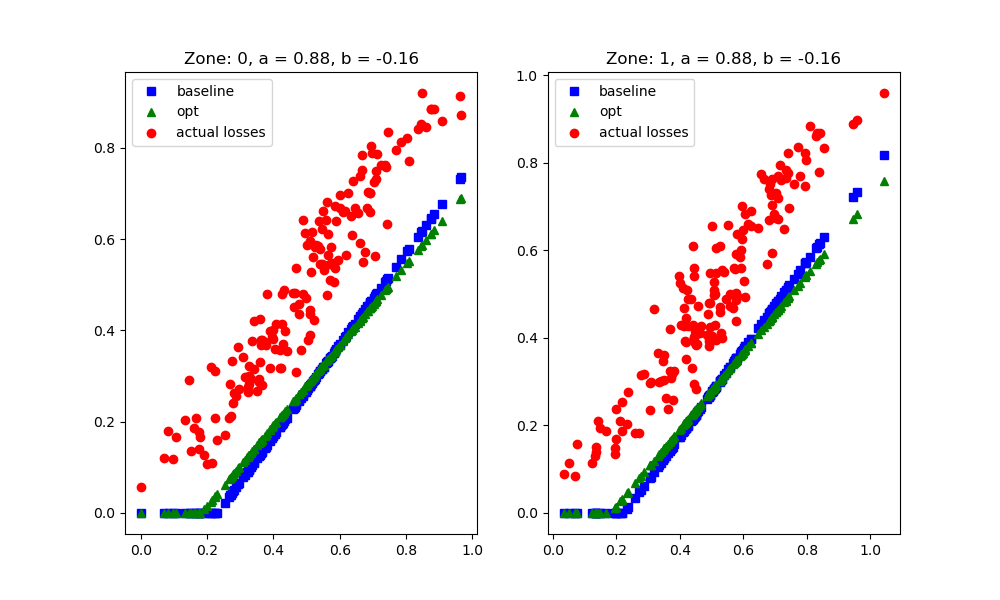
\includegraphics[width=0.75\textwidth]{../../output/figures/Logit_Bootstrap/no_corr_linear_premium.png}
            \caption{No Correlation, model correctly specified. These are graphs of the payment schedules of the insurance contracts for the two zones. The green payment schedule is for the contract designed by our method, labeled ``opt''. The blue payment schedule is for the baseline contracts, labeled ``baseline''. The red dots are the farmer losses. $a$ is the slope of the payout of our contract, and $b$ is the deductible of our contract.}
        \end{figure}

        \begin{table}[H]
            \centering
            % \small
            \begin{tabular}{lllllll}
\toprule
   Model &      Max CVaR &       Max VaR &  Max SemiVar & $|VaR_2 - VaR_1|$ & Required Capital &  Average Cost \\
\midrule
Baseline &          0.27 &          0.29 &         0.24 &              0.03 &             0.65 &          0.67 \\
         &   [0.23, 0.4] &  [0.25, 0.42] &  [0.18, 0.3] &       [0.0, 0.15] &     [0.53, 0.82] &  [0.52, 0.74] \\
     Opt &          0.29 &          0.29 &         0.21 &              0.01 &             0.58 &          0.67 \\
         &  [0.25, 0.37] &  [0.25, 0.36] & [0.14, 0.27] &       [0.0, 0.03] &     [0.47, 0.74] &  [0.51, 0.74] \\
    Diff &         -0.01 &          0.01 &         0.03 &              0.02 &             0.06 &          0.00 \\
         & [-0.03, 0.05] & [-0.01, 0.07] & [0.01, 0.08] &     [-0.02, 0.13] &     [0.04, 0.09] & [-0.01, 0.01] \\
\bottomrule
\end{tabular}

            \caption{Performance Metrics. The values shown correspond to the median value of the metric across 1000 simulation. The intervals shown are the $5^{th}$ and $95^{th}$ percentile values of the metrics.}
        \end{table}
        \FloatBarrier


        \paragraph{Positive Correlation Case} Under the insurance contracts designed by our model, farmers have a slightly lower probability of having a net loss that exceeds the specified threshold. Furthermore, the difference between the average losses between the two zones is significantly smaller relative to the baseline. The contracts designed by our model require $14\%$ less capital than the baseline contracts. The costs of the two contracts are basically equivalent. 
        \begin{figure}[H]
            \centering
            % \caption{Positive Correlation, model correctly specified}
            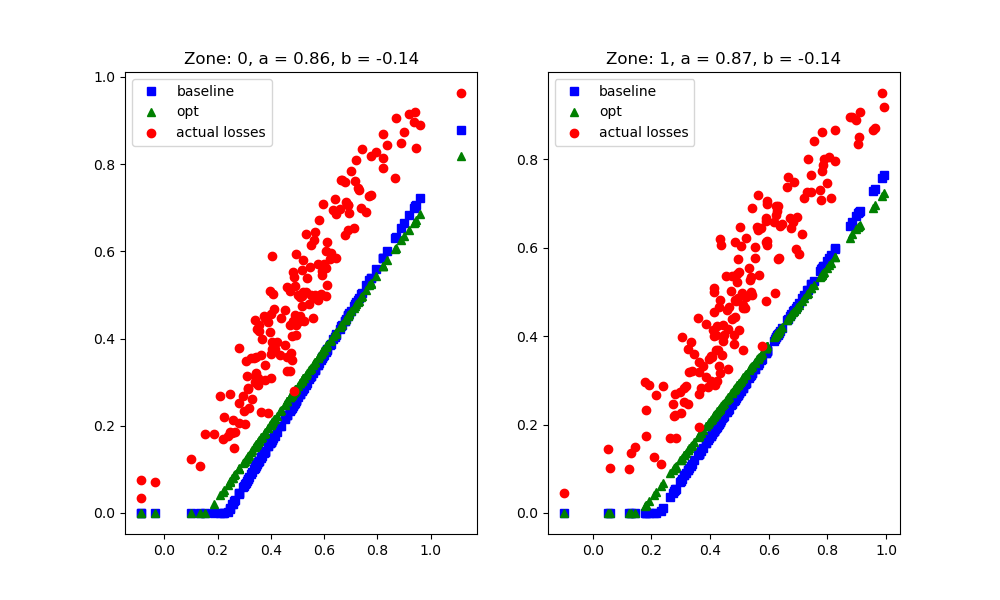
\includegraphics[width=0.75\textwidth]{../../output/figures/Logit_Bootstrap/pos_corr_linear_premium.png}
            \caption{Positive Correlation, model correctly specified. These are graphs of the payment schedules of the insurance contracts for the two zones. The green payment schedule is for the contract designed by our method, labeled ``opt''. The blue payment schedule is for the baseline contracts, labeled ``baseline''. The red dots are the farmer losses. $a$ is the slope of the payout of our contract, and $b$ is the deductible of our contract.}
        \end{figure}

        \begin{table}[H]
            \centering
            % \small
            
            \begin{tabular}{lllllll}
\toprule
   Model &       Max CVaR &      Max VaR &  Max SemiVar & $|VaR_2 - VaR_1|$ & Required Capital & Average Cost \\
\midrule
Baseline &           0.61 &         0.64 &         0.02 &              0.01 &             0.88 &         0.82 \\
         &   [0.59, 0.65] & [0.62, 0.66] & [0.01, 0.03] &       [0.0, 0.03] &      [0.72, 1.1] & [0.68, 0.96] \\
     Opt &           0.65 &         0.65 &         0.01 &              0.01 &             0.74 &         0.52 \\
         &   [0.63, 0.68] & [0.62, 0.67] &  [0.0, 0.02] &       [0.0, 0.03] &      [0.6, 0.98] & [0.44, 0.59] \\
    Diff &          -0.03 &        -0.01 &         0.01 &              0.00 &             0.13 &         0.31 \\
         & [-0.06, -0.02] & [-0.02, 0.0] &  [0.0, 0.01] &     [-0.02, 0.02] &     [0.09, 0.17] & [0.18, 0.43] \\
\bottomrule
\end{tabular}

            \caption{Performance Metrics. The values shown correspond to the median value of the metric across 1000 simulation. The intervals shown are the $5^{th}$ and $95^{th}$ percentile values of the metrics.}
        \end{table}
        \FloatBarrier

        \paragraph{Negative Correlation Case} Under the insurance contracts designed by our model, farmers have a slightly lower probability of having a net loss that exceeds the specified threshold. Furthermore, the difference between the average losses between the two zones is significantly smaller relative to the baseline. The contracts designed by our model require $11\%$ less capital than the baseline contracts. The costs of the two contracts are practically equivalent. 
        \begin{figure}[H]
            \centering
            % \caption{Negative Correlation, model correctly specified}
            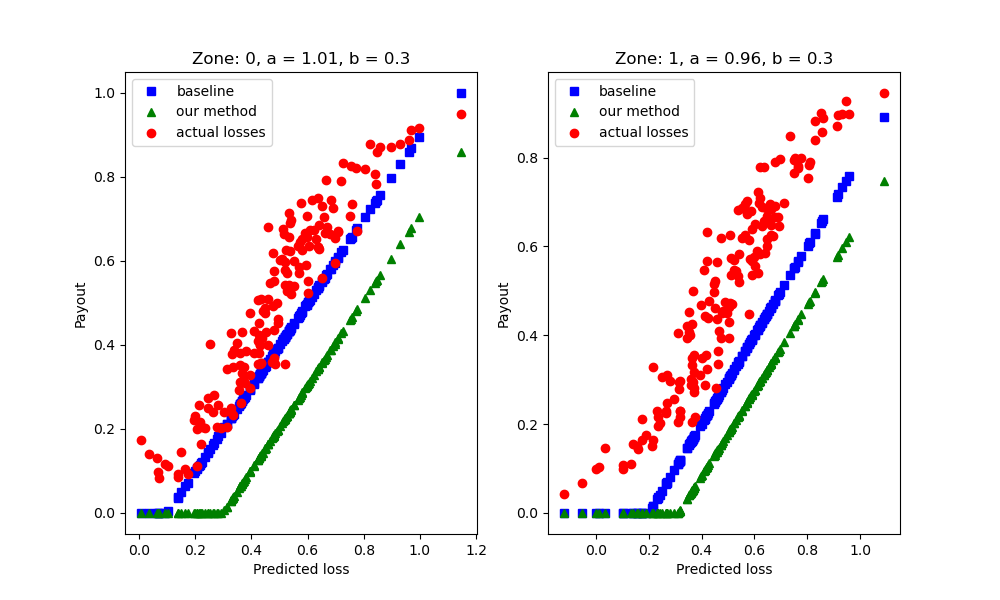
\includegraphics[width=0.75\textwidth]{../../output/figures/Logit_Bootstrap/neg_corr_linear_premium.png}
            \caption{Negative Correlation, model correctly specified. These are graphs of the payment schedules of the insurance contracts for the two zones. The green payment schedule is for the contract designed by our method, labeled ``opt''. The blue payment schedule is for the baseline contracts, labeled ``baseline''. The red dots are the farmer losses. $a$ is the slope of the payout of our contract, and $b$ is the deductible of our contract.}
        \end{figure}

        \begin{table}[H]
            \centering
            \small
            \caption{Performance Metrics. The values shown correspond to the median value of the metric across 1000 simulation. The intervals shown are the $5^{th}$ and $95^{th}$ percentile values of the metrics.}
            \begin{tabular}{lllllll}
\toprule
   Model &       Max CVaR &       Max VaR &  Max SemiVar & $|VaR_2 - VaR_1|$ & Required Capital & Average Cost \\
\midrule
Baseline &           0.57 &          0.59 &         0.03 &              0.01 &             0.30 &         0.75 \\
         &   [0.54, 0.59] &  [0.57, 0.61] & [0.02, 0.06] &       [0.0, 0.05] &     [0.24, 0.38] &  [0.6, 0.85] \\
     Opt &           0.60 &          0.60 &         0.02 &              0.01 &             0.29 &         0.47 \\
         &   [0.57, 0.63] &  [0.59, 0.63] & [0.01, 0.04] &       [0.0, 0.04] &     [0.23, 0.38] & [0.41, 0.52] \\
    Diff &          -0.03 &         -0.01 &         0.01 &              0.00 &             0.02 &         0.29 \\
         & [-0.05, -0.01] & [-0.03, -0.0] &  [0.0, 0.02] &     [-0.02, 0.02] &    [-0.08, 0.07] &  [0.14, 0.4] \\
\bottomrule
\end{tabular}

        \end{table}
        \FloatBarrier

      \subsubsubsection{Incorrectly specified prediction model}
        \paragraph{No correlation Case} The insurance contracts designed by our model provide a similar level of protection as the baseline contracts, at a cost that is $6\%$ lower. However, the average losses are slightly less equitable. The capital requirements for our contracts are $4.9\%$ lower than the baseline. 
        \begin{figure}[H]
            \centering
            % \caption{No Correlation, model misspecified}
            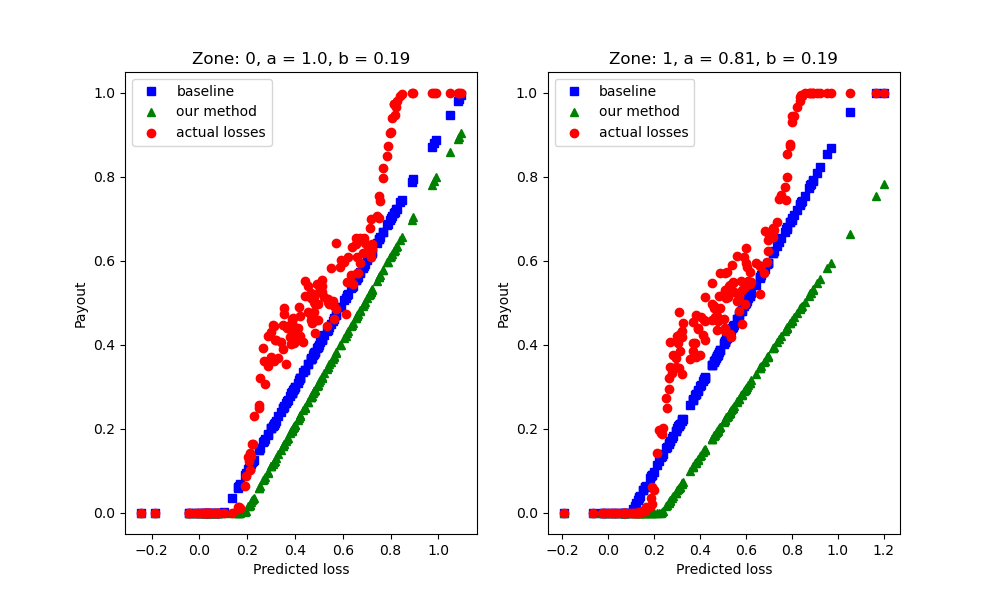
\includegraphics[width=0.75\textwidth]{../../output/figures/Logit_Bootstrap/no_corr_nonlinear_premium.png}
            \caption{No Correlation, model misspecified. These are graphs of the payment schedules of the insurance contracts for the two zones. The green payment schedule is for the contract designed by our method, labeled ``opt''. The blue payment schedule is for the baseline contracts, labeled ``baseline''. The red dots are the farmer losses. $a$ is the slope of the payout of our contract, and $b$ is the deductible of our contract.}
        \end{figure}

        \begin{table}[H]
            \centering
            % \small
            
            \begin{tabular}{lllllll}
\toprule
   Model &     Max CVaR &       Max VaR &   Max SemiVar & $|VaR_2 - VaR_1|$ & Required Capital & Average Cost \\
\midrule
Baseline &         0.65 &          0.67 &          0.02 &              0.02 &             0.70 &         0.91 \\
         &  [0.6, 0.84] &  [0.61, 0.77] &  [0.01, 0.08] &       [0.0, 0.07] &     [0.21, 0.93] &  [0.7, 0.97] \\
     Opt &         0.71 &          0.67 &          0.03 &              0.02 &             0.61 &         0.56 \\
         & [0.64, 0.86] &  [0.61, 0.77] &  [0.01, 0.08] &       [0.0, 0.08] &      [0.0, 0.86] &  [0.0, 0.74] \\
    Diff &        -0.04 &         -0.00 &         -0.00 &             -0.00 &             0.10 &         0.36 \\
         & [-0.1, 0.02] & [-0.02, 0.06] & [-0.03, 0.02] &     [-0.03, 0.03] &    [-0.03, 0.26] & [0.18, 0.81] \\
\bottomrule
\end{tabular}

            \caption{Performance Metrics. The values shown correspond to the median value of the metric across 1000 simulation. The intervals shown are the $5^{th}$ and $95^{th}$ percentile values of the metrics.}
        \end{table}
        \FloatBarrier


        \paragraph{Positive Correlation Case} The insurance contracts designed by our model provide a slightly worse level of protection as the baseline contracts, at a cost that is $11\%$ lower. However, the capital requirements for our contracts are $5.7\%$ higher than the baseline. 
        \begin{figure}[H]
            \centering
            % \caption{Positive Correlation, model misspecified}
            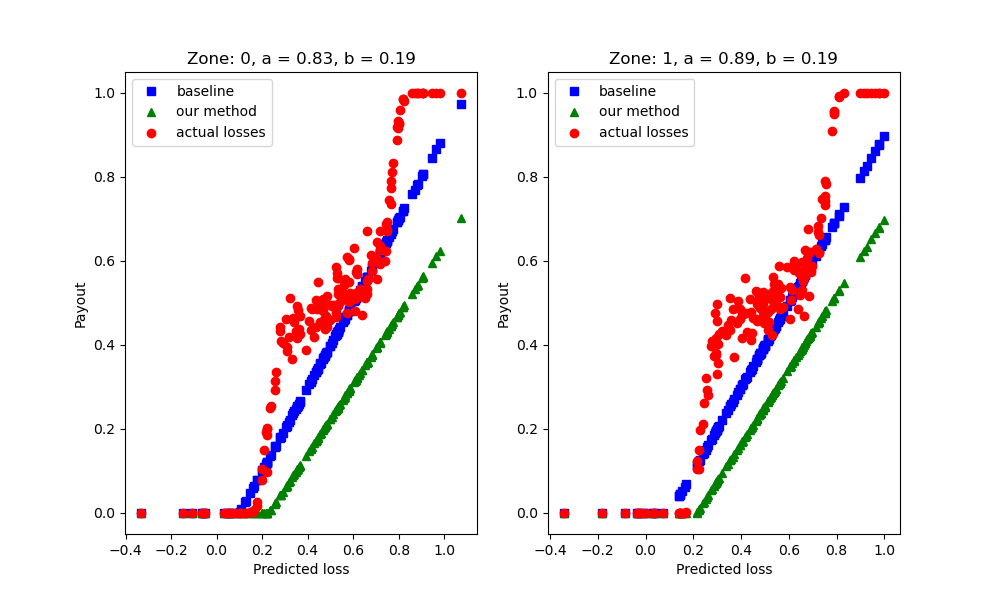
\includegraphics[width=0.75\textwidth]{../../output/figures/Logit_Bootstrap/pos_corr_nonlinear_premium.png}
            \caption{Positive Correlation, model misspecified. These are graphs of the payment schedules of the insurance contracts for the two zones. The green payment schedule is for the contract designed by our method, labeled ``opt''. The blue payment schedule is for the baseline contracts, labeled ``baseline''. The red dots are the farmer losses. $a$ is the slope of the payout of our contract, and $b$ is the deductible of our contract.}
        \end{figure}

        \begin{table}[H]
            \centering
            % \small
            
            \begin{tabular}{lllllll}
\toprule
   Model &      Max CVaR &      Max VaR &  Max SemiVar & $|VaR_2 - VaR_1|$ & Required Capital &  Average Cost \\
\midrule
Baseline &          0.50 &         0.48 &         0.13 &              0.02 &             0.90 &          0.66 \\
         &  [0.06, 0.68] & [0.06, 0.58] & [0.01, 0.58] &       [0.0, 0.39] &     [0.27, 1.12] &  [0.22, 1.16] \\
     Opt &          0.40 &         0.36 &         0.06 &              0.01 &             0.75 &          0.66 \\
         &   [0.1, 0.67] & [0.09, 0.53] & [0.01, 0.51] &       [0.0, 0.05] &     [0.09, 1.11] &  [0.22, 1.13] \\
    Diff &         -0.02 &         0.03 &         0.02 &              0.00 &             0.11 &          0.01 \\
         & [-0.06, 0.18] & [-0.04, 0.2] & [-0.02, 0.2] &     [-0.02, 0.37] &    [-0.07, 0.37] & [-0.02, 0.06] \\
\bottomrule
\end{tabular}

            \caption{Performance Metrics. The values shown correspond to the median value of the metric across 1000 simulation. The intervals shown are the $5^{th}$ and $95^{th}$ percentile values of the metrics.}
        \end{table}
        \FloatBarrier

        \paragraph{Negative Correlation Case} The insurance contracts designed by our model provide a similar level of protection as the baseline contracts, at a cost that is $7\%$ lower. The equity of the losses is similar with both contracts. The capital requirements for our contracts are $10\%$ lower than the baseline. 
        \begin{figure}[H]
            \centering
            % \caption{Negative Correlation, model misspecified}
            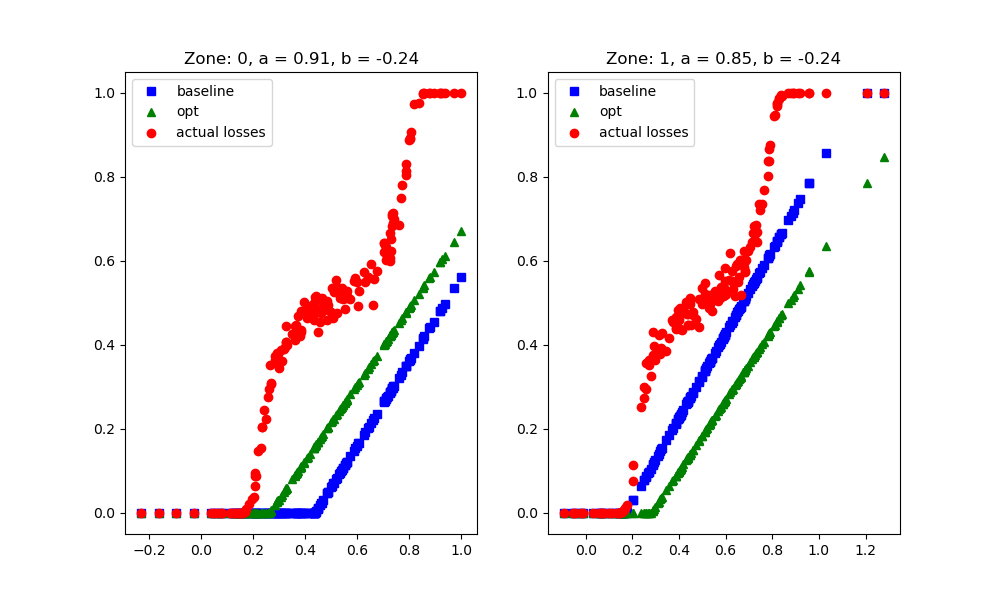
\includegraphics[width=0.75\textwidth]{../../output/figures/Logit_Bootstrap/neg_corr_nonlinear_premium.png}
            \caption{Negative Correlation, model misspecified. These are graphs of the payment schedules of the insurance contracts for the two zones. The green payment schedule is for the contract designed by our method, labeled ``opt''. The blue payment schedule is for the baseline contracts, labeled ``baseline''. The red dots are the farmer losses. $a$ is the slope of the payout of our contract, and $b$ is the deductible of our contract.}
        \end{figure}

        \begin{table}[H]
            \centering
            % \small
            
            \begin{tabular}{lllllll}
\toprule
   Model &      Max CVaR &       Max VaR &   Max SemiVar & $|VaR_2 - VaR_1|$ & Required Capital & Average Cost \\
\midrule
Baseline &          0.63 &          0.64 &          0.02 &              0.02 &             0.33 &         0.85 \\
         &  [0.57, 0.84] &  [0.59, 0.75] &  [0.01, 0.12] &       [0.0, 0.08] &     [0.11, 0.44] &  [0.67, 0.9] \\
     Opt &          0.66 &          0.64 &          0.03 &              0.02 &             0.33 &         0.53 \\
         &  [0.59, 0.86] &   [0.6, 0.73] &  [0.01, 0.12] &       [0.0, 0.06] &      [0.0, 0.42] &  [0.0, 0.71] \\
    Diff &         -0.03 &         -0.01 &         -0.00 &             -0.00 &             0.01 &         0.31 \\
         & [-0.07, 0.02] & [-0.02, 0.05] & [-0.02, 0.02] &     [-0.02, 0.02] &    [-0.09, 0.11] &  [0.13, 0.8] \\
\bottomrule
\end{tabular}

            \caption{Performance Metrics. The values shown correspond to the median value of the metric across 1000 simulation. The intervals shown are the $5^{th}$ and $95^{th}$ percentile values of the metrics.}
        \end{table}
        \FloatBarrier
  
  \subsection{Kenya Evaluation}
    \subsubsection{Data Sources}
    
    \subsubsection{Data Creation}

    \subsubsection{Evaluation Procedure}

    \subsubsection{Results}

\section{Discussion}
  In this paper we proposed a standardized approach to design index insurance products. Our proposed method provides more equitable and cost efficient protection, and can scale to more areas. We think there are many benefits to having a standardized, optimization based approach. For one, it can be easier to incorporate supply side constraints with regards to risk and overall cost. It can also make it easier to incorporate constraints regarding the quality of the product. Both of these are significant considerations when thinking about the large scale adoption of index insurance (\cite{jensen2017agricultural}). In the future, we hope to better incorporate uncertainty into the model, by using robust optimization. One of the factors that drives up the cost of index insurance is that there is often very little historical data for the insured regions, as a result, insurers add an uncertainty markup to protect themselves. Reinsurers behave similarly. We hope that by incorporating this data uncertainty into the problem, we can make a product that is less costly and more attractive to insurers and reinsurers. 

\printbibliography
\end{document}